\section{Brief History and Introduction}
Lambda-calculus and combinatory logic were initially invented in the early 20\textsuperscript{th} century as logic systems but later found applications as a computational model mirroring functional programs such as Lisp.

The first computationally intractable problems to be discovered were originally described not in terms of idealised computers, such as Turing machines, but in $\lambda$-calculus\cite{LambdaAndCombinatorsIntro}.

\begin{itemize}
    \event{1920}{Moses Schönfinkel invents combinatory logic}
    \event{1927}{American logician Haskell Brooks Curry independently rediscovers it and turns it into a workable system}
    \event{1932}{American logician Alonzo Church publishes the first paper on $\lambda$-calculus, {\it A Set of Postulates for the Foundation of Logic}}
    \event{1936}{Alan Turing conceives of the Turing Machine, which becomes the dominant model of computation in the field}
    \event{1958}{LISP, the first functional programming language, is created}
    \event{1973}{ML, which adds Robin Milner's type system onto Lisp, becomes the first statically typed functional language}
    \event{1990}{Haskell, named after American logician Haskell Curry, pioneers a number of advanced programming concepts, including lazy evaluation}
\end{itemize}
In a word, what makes a program functional is statelessness. In programming, a state is an environment external to a function which affects the way it works. In mathematics, this notion is counterintuitive because one always expects functions to give the same output for the same input because they can't mutate. By definition, one has

\begin{equation*}
    \forall f:A\rightarrow B,\ x,y\in A,\quad x=y \implies f(x)=f(y)
\end{equation*}

If you define $f(x) = 2x$, one always expects $f(3) = 6$. One does not expect $f$ to suddenly start tripling its inputs, for example. Even in situations where one requires a function to change, such as when converging pointwise or uniformly, a sequence is constructed with each term denoted $f_{n \in\mathbb{N}}$, effectively giving the function one more input. 

This is not the case in imperative programs, such as the following JavaScript code being run in a command line interpreter:

\begin{lstlisting}
    > var n = 2;
    > function f(x) {
        return n*x;
      }
    > f(3)
    6
    > f(5)
    10
    > function set_n(m) {
        n = m;
      }
    > set_n(4)
    undefined
    > f(3)
    12
    > f(5)
    20
\end{lstlisting}

Let's start by examining the first two statements. We defined a variable $n=2$ and then a function $f$. We confirm it behaves the same way as our mathematically defined $f$ on the next couple of lines by running \code{f(3)} and \code{f(5)} to get the expected outputs. We then proceed to define $function set_n(m)$ which, despite its declaration, does not behave like a mathematical function at all as it does not map one value to another. Instead, it executes the statement \code{n = m}, which is an instruction assigning the value of \code{m} to the variable \code{n}.

This variable is a simple example of state, demonstrating two properties which functions in programs can have but those in mathematics cannot:

\begin{itemize}
    \item indeterminism - the inability to know the output of a function solely from the input. This is shown by \code{function f(x)}.
    \item side effects - the modification of some variable outside of those given to the function. This is done by \code{function set\_n(m)}.
\end{itemize}

There are, of course, functions which exhibit both properties but, in any case, a function interacting with some kind of external state not included in the input arguments is called "impure". One which merely maps an input to an output as per the mathematical definition, on the other hand, {\it is} pure.

Why should one care about functional purity? A deterministic function is, by definition, 100\% reliable, allowing a greater degree of modularisation of code\cite{WhyFunctional}. This does not merely refer, as Hughes writes, to organising a program into multiple files or library modules. It isn't difficult to split code of either paradigm, functional or imperative, into a few monolithic chunks.
Rather, a functional program can be split much more finely, as it naturally encourages a bottom-up style as described in the introduction of {\it On Lisp}. In this book, Paul Graham explains how a lisp program can be naturally layered from small, standalone pieces of code\footnote{Graham mainly focuses on macros as granting this capability but those, in fact, work because Lisp is functional. In any case, macros are beyond the scope of this essay and Lisp would still retain, as other functional languages do, a great deal of its power without them.}. This is because pure functions are entirely self-contained and easily testable. All one needs is a checklist of pairs of inputs and outputs without concern of the state of the environment in which that function is being tested.

The reason we study $\lambda$-calculus, combinators, and monads in this paper is that these form a model of computation which mirrors a functional program. For comparison, we shall first look at a model which mirrors an imperative program - the Turing Machine.

\subsection{The Turing Machine and Imperative Programming}
The Turing Machine (TM) is a hypothetical device equipped with a tape divided into an infinite number of cells along its length. The TM performs computations by manipulating symbols occupying each cell.
\begin{figure}[h]
    \centering
    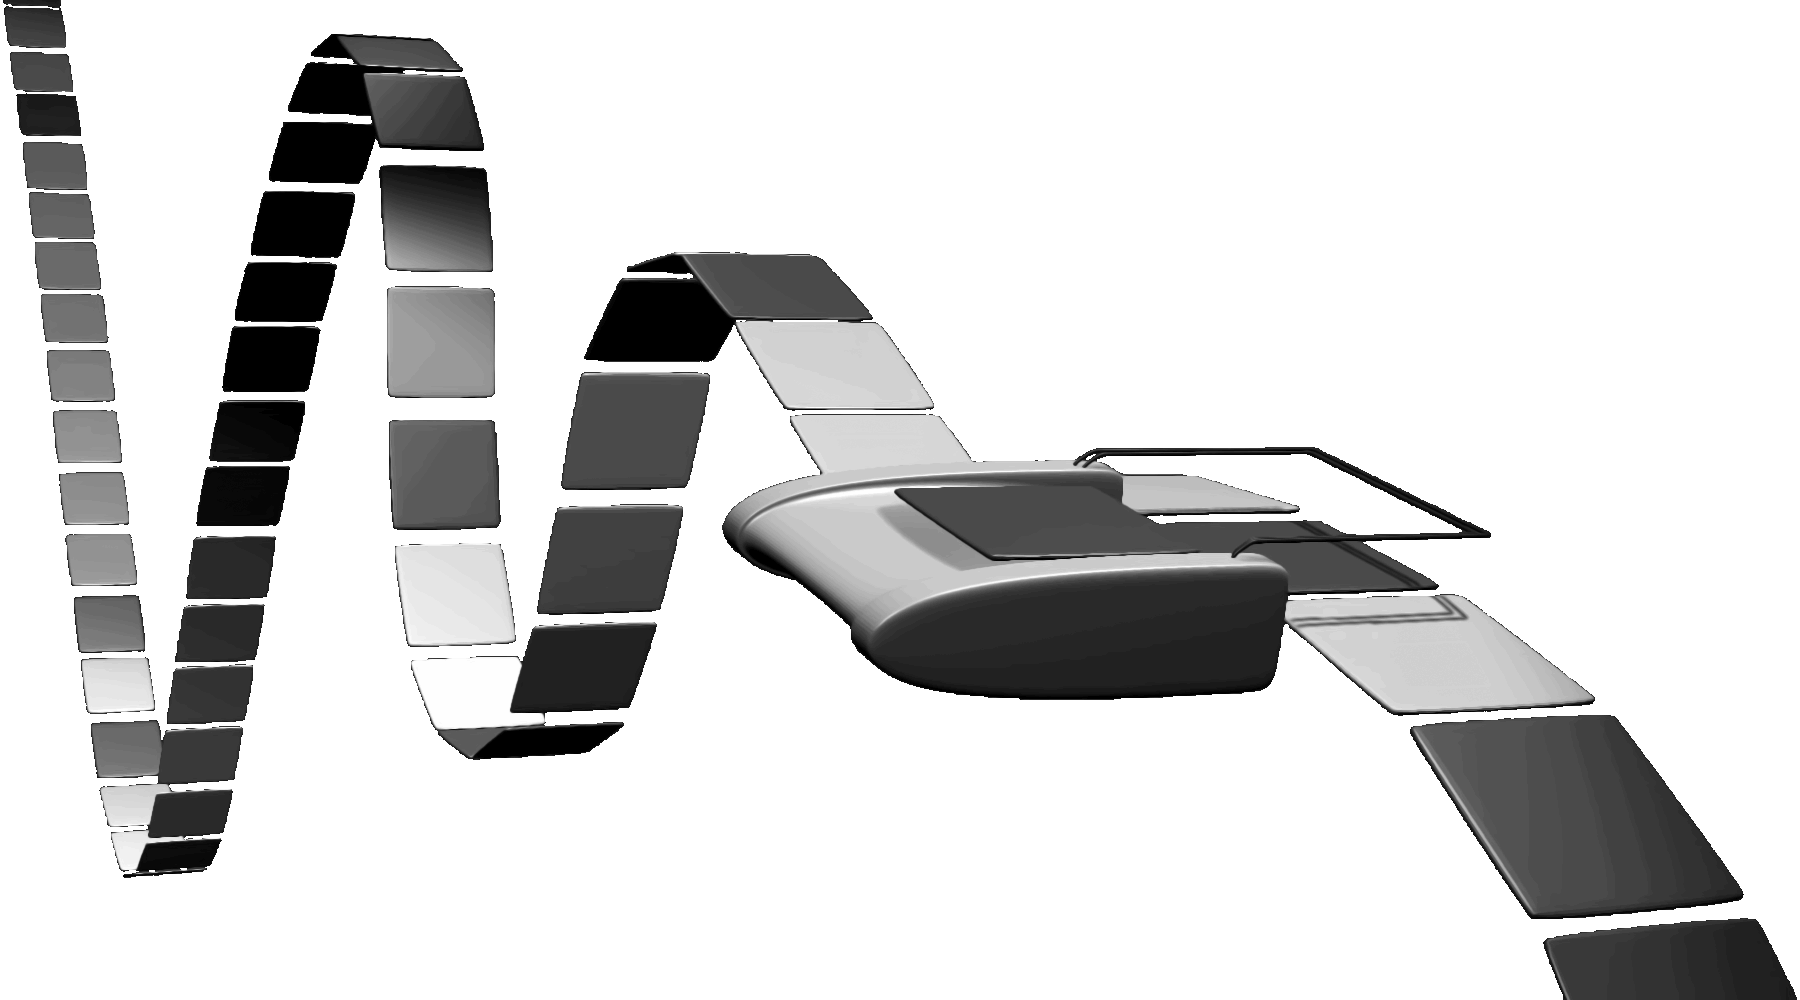
\includegraphics[width=6cm]{turing_machine}
    \caption{An artistic impression of a Turing Machine}
\end{figure}

A formal definition of one is given by Hopcroft and Ullman in their book on theory of automata\cite{IntroToAutomata} as a 7-tuple but, for our purposes, a simpler model with just 4 ingredients shall suffice. Define a Turing Machine as a 4-tuple $(Q, \Gamma, F, \delta)$ where:

\begin{itemize}
    \item $Q$ is a finite, non-empty set of conditions\footnote{Other literature usually refers to these "conditions" as "states". We change the name to avoid confusion with the subtly different notion of "state" we discuss here. That notion is some environment external to a function which affects or is affected by it without being explicitly passed as input.}
    \item $\Gamma$ is a finite, non-empty alphabet of symbols. Each cell on the tape contains one of these symbols.
    \item $F \subset Q$ is a set of {\it final} or {\it accepting} conditions. Upon encountering one of these, the TM finishes its work, leaving the final state of the type to be read off as output.
    \item $\delta: (Q - F) \times \Gamma \rightarrow I$, a mapping from the set of all possible pairs of non-final conditions and symbols to an instruction. It can be thought of as a table of instructions with a column for each condition and a row for each symbol.
    \item $I = \Gamma \times \{L, R\} \times Q$ is the set of all possible instructions this TM could accept. An instruction is a triple of the following things:
        \begin{enumerate}
            \item Replace the symbol in the current cell with any other symbol from the alphabet.
            \item Move the head one space to the left or right.
            \item Change the current (non-final) condition to any condition in Q.
        \end{enumerate}
\end{itemize}

The TM has a head for reading/writing symbols which is positioned over one cell. It operates by reading the value of that cell and feeding that to the function $\delta$ along with its current state and executing the given instruction. This process is repeated until one of the {\it final conditions} from $F$ are reached.

The model of the Turing Machine proved to be a useful advancement. It naturally led to the concept of Turing Completeness which is the ability of a logic system to simulate a Turing Machine\cite{TuringEnigma}. This property is now a widely accepted standard to which a programming language must measure up in order to be considered practically usable. Another advancement is proving the undecidability of the halting problem - the fact that there cannot exist a computer program which can accept another arbitrary program as input and determine whether that program will eventually terminate for a given input.

In relation to programming, the Turing Machine can be thought of as physical representation of the entities present in imperative code, with each cell corresponding to a variable, the alphabet of symbols to the values those variables can take, and each instruction to an assignment statement such as the \code{n = m} in our JavaScript example. The sequence of symbols stored in the tape (along with the currently stored condition), represents the state of the program at a given time.

If the TM is a stateful model of computation, this invites the question of what a stateless one would look like. This is what the $\lambda-calculus$ and combinatory logic we shall look at later provides.

\subsection{Statelessness via Functional Programming}
A computation is merely the mapping of some input to an appropriate output, which exactly matches the notion of a function. A model of one can therefore be built from a system of rules which describes how simpler functions can be combined into larger ones, which is precisely what the combinatory logic developed by Schönfinkel and Curry and the lambda-calculus developed by Alonzo Church does. We shall explore this further in section 3.1 below.

Functional programming is a way of designing languages and writing code which treats functions as data, putting them on the same footing as strings, numbers, etc. This introduces the idea of "higher-order functions", which accept other functions as inputs.

Moreover, languages such as Haskell are said to treat functions as "first-class citizens" - they are declared using the same syntax as concrete pieces of data such as numbers and strings. Indeed, such data can be merely thought of as functions that accept no arguments and so always return a constant value.

\subsection{Functional Languages}
The concept of functional programming is nothing new. The second programming language ever invented, LISP, is functional. LISP was created by MIT's Artificial Intelligence Group to experiment with giving machines the ability to handle declarative as well as imperative statements\cite{RecursiveFunctions}.

A declaration, as opposed to an imperative statement, is one which defines some word or expression as opposed to giving a machine a direct instruction. Such declarations are then used as references by the machine to understand further usage of the defined words/expressions in other points in the program. Expressing a program in terms of such declarations results in the statelessness we talked about earlier because a list of definitions can be written in any order. A list of instructions, in contrast, has to be performed sequentially in order to ensure correct manipulation of state.

This lack of order is taken advantage of in functional programming to break it up into independent units which can be mixed and matched as a coder desires - the kind of modularisation talked about by Graham\cite{OnLisp} and Hughes\cite{WhyFunctional} we mentioned in the introduction.

Since LISP, many other programming languages have been developed which introduced other advancements on top of statelessness. 15 years later, ML became the first statically typed functional language. Static typing is the checking of function signatures at compile time, ensuring that integers, fractions, letters, boolean values, etc are all in their proper place, reducing the likelihood of errors when running a program.

Such type checking requires a formal system of logic, which was built into Church's $\lambda$-calculus by J Roger Hindley and Robin Milner. This type system continues to be used in Haskell, the language with which we shall illustrate the mathematics in this paper. Haskell has a certain syntactic purity not seen in many other languages, requiring no keywords such as \code{def} or \code{function} in order to define a function. To see this, let's look at this code which computes the hypotenuse of a right-angled triangle:
\begin{lstlisting}
    hypot a b = sqrt (a*a + b*b)
\end{lstlisting}
and compare it to the equivalent code in Python:
\begin{lstlisting}
    def hypot(a, b):
        return sqrt(a*a + b*b)
\end{lstlisting}
which has a lot more unnecessary syntactic clutter by way of parentheses, colons, and $return$s. In this way, Haskell's syntax is much closer to mathematical notation and lends itself much better to illustrating the concepts explored in this paper.

Why go functional as opposed to imperative? The reason is productivity. The fields of lambda, combinators, and categories provide a more natural language to express many computational concepts that gives functional code these advantages:
\begin{itemize}
    \item Expressiveness - provide given functionality with terser source code.
    \item Correctness - catch more errors during compile time, reducing run time bugs.
\end{itemize}
As explained earlier, functional programming introduces the idea of functions as first class citizens - treating them as pieces of data on an equal footing with numbers, strings, booleans, etc. This allows functions to be return values and arguments of other functions. In the latter case, those functions which accept other functions as arguments are referred to as being "higher order".

Why is it useful for a function to be higher order? We encounter examples of such functions all the time in mathematics, though they are typically referred to as operators. Consider this Haskell code for numerically approximating the differential operator:
\begin{lstlisting}
    deriv f x = (f (x + h) - f x) / h
        where h = 0.001
\end{lstlisting}
The higher order function is called \code{deriv} and takes 2 arguments, the function $f$ we are differentiating and the point $x$ at which we want the gradient. We also define an arbitrary step size $h$ which regulates the precision of the value we get.

What this means is that, in the functional style, one combines simple functions into more complex ones by putting them together in a similar manner to how one would assemble a Lego model from smaller and smaller modules which are ultimately made out of bricks.

Furthermore, just as Lego parts have these bumps and divots which slot very particularly into one another to hold a model together, the theories of lambda calculus and combinatory logic provide a rigorous framework which describes precisely how larger functions can be built from smaller ones to ensure correctness of a program.